%------------------------------------------------------------------------------------------------
%PAGINA 11
\fancyhf{}
\fancyhead[r]{\thepage} 
\begin{center}
{\fontsize{13}{16}\selectfont \textbf{SISTEMA}}
\end{center}
\vspace{0.5cm}

{\fontsize{13}{15}\selectfont
... tienen una \textbf{configuración espacial}, ya que están compuestos por seres vivos que se encuentran en relaciones espaciales definidas entre sí.) Todo sistema tiene tanto una \textbf{estructura de sistema} (o vínculo) como una \textbf{estructura espacial} (o configuración). Por otro lado, los agregados o ensamblajes tienen estructuras espaciales pero carecen de estructuras de sistema.

Para facilitar la referencia, reunimos algunas de las anteriores aclaraciones en la

\textbf{DEFINICIÓN 1.5} Sea $\sigma''$ un sistema concreto con A-estructura $\mathcal{S}_A(\sigma'', t)$ en el momento $t$. Entonces
(i) la \textbf{estructura A-interna} de $\sigma''$ en $t$ es el subconjunto de $\mathcal{S}_A(\sigma'', t)$ compuesto por las relaciones entre las A-partes de $\sigma''$ en $t$;
(ii) la \textbf{configuración} (o \textbf{estructura espacial}) de $\sigma''$ en $t$ es el subconjunto de $\mathcal{S}_A(\sigma'', t)$ compuesto por las relaciones espaciales entre las A-partes de $\sigma''$ en $t$.

\subsection*{1.4. Subsistema}
Un componente de un sistema puede o no ser un sistema en sí mismo. Si lo es, lo llamamos \textbf{'subsistema'}. Más explícitamente, establecemos la

\textbf{DEFINICIÓN 1.6} Sea $\sigma''$ un sistema con composición $\mathcal{C}(\sigma'', t)$, entorno $\mathcal{E}(\sigma'', t)$ y estructura $\mathcal{S}(\sigma'', t)$ en el momento $t$. Entonces una cosa $x$ es un subsistema de $\sigma''$ en $t$, o $x \triangleleft \sigma''$, si y solo si
(i) $x$ es un sistema en el momento $t$, y
(ii) $\mathcal{C}(x, t) \subseteq \mathcal{C}(\sigma'', t) \land \mathcal{E}(x, t) \supseteq \mathcal{E}(\sigma'', t) \land \mathcal{S}(x, t) \subseteq \mathcal{S}(\sigma'', t)$.

Por definición, la relación de subsistema ($\triangleleft$) es una \textbf{relación de orden}, es decir, es reflexiva, asimétrica y transitiva. Así, en particular, si $\sigma_1 \triangleleft \sigma_2$ y $\sigma_2 \triangleleft \sigma_3$, entonces $\sigma_1 \triangleleft \sigma_3$. Haremos uso de esta propiedad al definir la noción de un \textbf{sistema de sistemas anidados} (Definición 1.7).

\textbf{Ejemplo 1} Las fábricas, los hospitales y las escuelas constituyen subsistemas de cualquier sociedad moderna. Por otro lado, las personas que los componen no son en sí mismas sistemas sociales: son biosistemas.

\textbf{Ejemplo 2} Un feto es un subsistema de su madre; se convierte en un sistema por derecho propio después del nacimiento: antes de eso, no cae bajo ninguna de las leyes, naturales o sociales, que rigen para los sistemas independientes.

Los sistemas de diferente tipo tienen composiciones diferentes o estructuras diferentes. (Una diferencia en la composición induce una diferencia estructural, pero no al revés, como lo demuestra la existencia de isómeros, es decir, sistemas con la misma composición pero estructuras diferentes.) Sin embargo, todos los sistemas del mismo género parecen tener la misma \textbf{estructura general} o "plan general" —

%------------------------------------------------------------------------------------------------
%PAGINA 12
}
\newpage
\fancyhf{}
\fancyhead[l]{\thepage} 
\begin{center}
{\fontsize{13}{16}\selectfont \textbf{CAPÍTULO I}}
\end{center}
\vspace{0.5cm}

{\fontsize{13}{15}\selectfont
... disculpe el antropomorfismo. Por ejemplo, todos los átomos consisten en núcleos rodeados de electrones, todos los sólidos son retículos atómicos o iónicos habitados por electrones errantes, e incluso la \textbf{estructura general} del esqueleto y los órganos es la misma para todos los vertebrados. (Sin embargo, la caracterización precisa de la noción de \textbf{estructura general} es un problema abierto.)

A menudo se dice que las estructuras vienen superpuestas o \textbf{anidadas} como sistemas de cajas chinas. Así, se dice que un polipéptido tiene dos estructuras, una \textbf{primaria} o básica (la secuencia lineal de aminoácidos), la otra \textbf{secundaria} y consistente en la configuración de la bobina completa. La configuración helicoidal de la molécula de ADN es un ejemplo de estructura secundaria. A su vez, la estructura secundaria puede determinar una \textbf{estructura terciaria}, por ejemplo, el plegamiento de toda la doble hebra en una configuración regular. Véase la Figura 1.3.

Desde nuestro punto de vista, no existe tal cosa como una \textbf{jerarquía de estructuras}. (Etimológicamente, 'jerarquía' significa un conjunto de componentes sagrados ordenados por una relación de poder o dominación.) Lo que sí tenemos aquí es un \textbf{sistema de sistemas anidados}, es decir, una colección de sistemas en la que cada uno es un subsistema de un sistema más grande (o supersistema). Y lo que los biólogos moleculares llaman 'estructura primaria' es la estructura del sistema más interno o \textbf{núcleo}, la estructura secundaria es la estructura del siguiente supersistema, y así sucesivamente. Esta noción es aclarada por la

\textbf{DEFINICIÓN 1.7} Sea $\sigma''$ un sistema y llamemos $\mathcal{T}$ a la totalidad de los sistemas, y
$$ \mathcal{M}_{\sigma} = \{\sigma_i \in \mathcal{T} \mid \sigma'' \triangleleft \sigma_i \land 1 \le i \le n\} $$
una colección de supersistemas de $\sigma''$ parcialmente ordenados por la relación de subsistema $\triangleleft$. Entonces
(i) $\mathcal{M}_{\sigma}$ es un \textbf{sistema de sistemas anidados} con núcleo $\sigma''$;

\begin{figure}[h!]
    \centering
    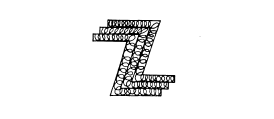
\includegraphics[width=0.6\textwidth]{imagenes/figura1.3.png}
    \caption*{Fig. 1.3. Un sistema imaginario de cajas chinas o jerarquía de sistemas. La estructura primaria, es decir, la secuencia de aminoácidos, no se muestra. La estructura secundaria es la hélice, la terciaria es la forma de Z. Y la estructura cuaternaria es la forma en que los individuos en forma de Z se ensamblan juntos, es decir, la doble escalera.}
\end{figure}
}

%------------------------------------------------------------------------------------------------
%PAGINA 13

\newpage
\fancyhf{}
\fancyhead[r]{\thepage} 
\begin{center}
{\fontsize{13}{16}\selectfont \textbf{SISTEMA}}
\end{center}
\vspace{0.5cm}

{\fontsize{13}{15}\selectfont
(ii) la \textbf{estructura primaria} de $\sigma$ es la estructura de $\sigma$ misma; la \textbf{estructura secundaria} de $\sigma$ es la estructura del supersistema más pequeño de $\sigma$ en $\mathcal{M}_{\sigma}$, es decir, $\sigma_1$; en general, la \textbf{estructura $n$-aria} de $\sigma$ es la estructura de $\sigma_{n-1}$.

\subsection*{1.5. Nivel}
Se ha hablado con frecuencia de \textbf{niveles de organización} (o complejidad, integración o evolución) y de una jerarquía de estos en la ciencia, particularmente en biología, durante el último medio siglo. Desafortunadamente, no hay consenso sobre el significado de los términos '\textbf{nivel}' y '\textbf{jerarquía}', que se utilizan de diversas maneras y rara vez, o nunca, se definen (Bunge, 1959b, 1959c). Esta vaguedad debe atribuirse no solo a los científicos, sino también a los filósofos: a los filósofos inexactos que desprecian la claridad y a los exactos que no son conscientes de los problemas filosóficos planteados por la investigación científica.

Intentemos remediar esta situación aclarando un concepto de \textbf{nivel} y el concepto correspondiente de \textbf{jerarquía} que son ampliamente utilizados en la ciencia contemporánea.

La idea intuitiva es simple: las cosas en cualquier nivel dado están compuestas por cosas que pertenecen a los niveles precedentes. Así, las biosferas están compuestas por ecosistemas, que están compuestos por poblaciones, que están compuestas por organismos, que están compuestos por órganos, que están compuestos por células, que están compuestas por orgánulos, que están compuestos por moléculas, que están compuestas por átomos, que están compuestos por las llamadas partículas elementales. Una forma de precisar esta noción es mediante la

\textbf{DEFINICIÓN 1.8} Sea $\mathcal{L} = \{L_i \mid 1 \le i \le n\}$ una familia de $n$ conjuntos no vacíos de cosas concretas. Entonces
(i) un nivel \textbf{precede} a otro si todas las cosas en este último están compuestas por cosas en (algunos o todos) de los primeros. Es decir, para cualquier $L_i$ y $L_j$ en $\mathcal{L}$,
$$ L_i < L_j =_{df} (\forall x)[x \in L_j \Rightarrow (\exists y) (y \in L_i \land y \in \mathcal{P}(x))] ; $$
(ii) una cosa pertenece a un nivel dado si está compuesta por cosas en (algunos o todos) los niveles precedentes. Es decir, para cualquier $L_i \in \mathcal{L}$:
$$ \forall x \text{ en } L_i : x \in L_i =_{df} \mathcal{P}(x) \subset \bigcup_{k=1}^{i-1} L_k ; $$
(iii) $\mathfrak{L} = \langle \mathcal{L}, < \rangle$ es una \textbf{estructura de nivel}.

Nótese lo siguiente. Primero, un \textbf{nivel no es una cosa sino un conjunto} y, por lo tanto, un concepto, aunque no uno ocioso. Por ende, los niveles no pueden actuar unos sobre otros. En particular, los niveles superiores no pueden mandar ni siquiera obedecer a los
}
%------------------------------------------------------------------------------------------------
%PAGINA 14
\newpage
\fancyhf{}
\fancyhead[L]{\thepage} 
\begin{center}
{\fontsize{13}{16}\selectfont \textbf{CAPÍTULO I}}
\end{center}
\vspace{0.5cm}

{\fontsize{13}{15}\selectfont
... inferiores. Toda mención de acción entre niveles es elíptica o metafórica, no \textbf{literal}. Segundo, la relación entre niveles no es ni la relación parte-todo ni la relación de inclusión de conjuntos, sino una relación \textbf{sui generis} definible en términos de las anteriores. Tercero, no hay nada oscuro en la noción de \textbf{precedencia de nivel} siempre que uno se adhiera a la definición anterior en lugar de interpretar '$L_i < L_j$' como "los $L_i$ son inferiores a los $L_j$" o algo similar. Cuarto, es erróneo llamar \textbf{jerarquía} a una estructura de nivel $\mathfrak{L} = \langle \mathcal{L}, < \rangle$, porque el orden de nivel $<$ no es una relación de dominio (Bunge, 1973a). Quinto, nuestro concepto es hasta ahora estático: no estamos asumiendo nada sobre el origen o el modo de composición de los sistemas en términos de evolución.

\subsection*{1.6. Asociación de Sistemas}
Ya sea que dos cosas formen o no un sistema, se puede asumir que se \textbf{asocian} (o se suman físicamente) para formar una tercera cosa. Así, la cosa $a$ y la cosa $b$, sin importar cuán distantes e indiferentes sean, pueden asumirse que forman la cosa $c = a + b$. En otras palabras, el conjunto de cosas es cerrado bajo la operación $+$ de asociación, adición física o yuxtaposición (Vol. 3, Cap. 1, Sec. 1).

No ocurre lo mismo con los sistemas: dos sistemas pueden o no asociarse para formar un tercero. Así, dos moléculas pueden no combinarse para formar un sistema, y dos sistemas sociales pueden no fusionarse para formar un tercero. En general, la adición física o asociación de dos cosas será una cosa, pero no un sistema: la \textbf{sistemología no se conserva}. El entorno, la estructura y quizás incluso la composición de la cosa resultante son diferentes de la mera unión de las composiciones, entornos y estructuras parciales. Véase la Figura 1.4. En resumen, el conjunto de todos los sistemas no tiene \textbf{estructura algebraica} —ni siquiera la más modesta de un semigrupo. Pero, por supuesto, dado que los sistemas son cosas, cumplen con el \textbf{álgebra de cosas}. En particular, se asocian para formar otras cosas.
\begin{figure}[h!]
    \centering
    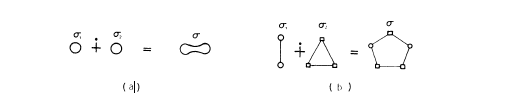
\includegraphics[width=0.6\textwidth]{imagenes/figura1.4.png}
    \caption*{Fig. 1.4. (a) Antes de la fusión, $\partial(\omega_1) = \{\omega_2\}$, $\partial(\omega_2) = \{\emptyset\}$. Después de la fusión, $\partial(\omega_1 + \omega_2) = \emptyset$. (b) Antes de la fusión, $\Psi(\omega_1) = \{\text{Enlace lineal}\}$ y $\Psi(\omega_2) = \{\text{Enlace triangular}\}$. Después de la fusión, $\Psi(\omega_1 + \omega_2) = \{\text{Enlace pentagonal}\}$.}
\end{figure}
%FALTA FIGURA 14

}
%------------------------------------------------------------------------------------------------
%PAGINA 15
\newpage
\fancyhf{}
\fancyhead[R]{\thepage} 
\begin{center}
{\fontsize{13}{16}\selectfont \textbf{SISTEMA}}
\end{center}
\vspace{0.5cm}

{\fontsize{13}{15}\selectfont
\subsection*{1.7. Otros Tipos de Sistemas: De Propiedades y Funcionales}
Estamos interesados no solo en sistemas concretos, sino también en \textbf{sistemas de propiedades}, o conjuntos de propiedades interrelacionadas, así como en \textbf{sistemas funcionales}, o conjuntos de procesos acoplados. Por ejemplo, la mayoría de las propiedades de una cosa, ya sea simple (básica) o un sistema, están ligadas entre sí; es decir, un cambio en una de ellas va acompañado de cambios en otras. Como consecuencia, la mayoría de los cambios que ocurren en una cosa simple o en un sistema están acoplados, de modo que si uno de ellos comienza o se detiene, otros cambian. (El prefijo cauteloso 'la mayoría' tiene la intención de excluir propiedades superficiales, como la posición y el color, que a menudo pueden cambiar considerablemente, dentro de ciertos límites, sin arrastrar cambios en otras propiedades.) Aunque toda cosa, aparte de un agregado o conglomerado, tiene propiedades y experimenta procesos que constituyen sistemas, los \textbf{sistemas de propiedades} y los \textbf{sistemas funcionales} son particularmente conspicuos entre los organismos. En particular, las capacidades mentales de un animal forman un sistema.

Utilizaremos las siguientes convenciones:

\textbf{DEFINICIÓN 1.9} Sea $p(x)$ el conjunto de propiedades de una cosa $x$, y $n(x)$ el conjunto de procesos que ocurren en $x$. Entonces
(i) el subconjunto $p_0(x) \subset p(x)$ es un \textbf{sistema de propiedades} de $x$ si y solo si toda propiedad en $p_0(x)$ está relacionada legalmente con al menos otra propiedad en $p_0(x)$;
(ii) el subconjunto $n_0(x) \subset n(x)$ es un \textbf{sistema funcional} de $x$ si y solo si todo proceso en $n_0(x)$ está relacionado legalmente con al menos otro proceso en $n_0(x)$.

Debido a que en un sistema todas las propiedades y procesos están legalmente interrelacionados, concluimos que, para todo $x$, $x$ es un sistema concreto si y solo si $p(x)$ es un sistema de propiedades o $n(x)$ es un sistema funcional.

\subsection*{1.8. Observaciones Finales}
La literatura sobre sistemas es \textbf{vasta}, está creciendo rápidamente y es algo \textbf{desconcertante}. (Cf. Klir y Rogers, 1977.) Sin embargo, el campo aún es \textbf{inmaduro} y su reputación está en peligro por un sector de charlatanes. Baste mencionar tres indicadores de inmadurez.

En primer lugar, la definición misma del concepto de sistema aún está en duda, por lo que muchos artículos comienzan dedicando tiempo a definir o redefinir el concepto. Sin embargo, tanto esfuerzo dedicado a las definiciones solo ha producido tres que son tan populares como incorrectas. Según la primera definición,
}

%------------------------------------------------------------------------------------------------
%PAGINA 16
\newpage
\fancyhf{}
\fancyhead[l]{\thepage} 
\begin{center}
{\fontsize{13}{16}\selectfont \textbf{CAPÍTULO 1}}
\end{center}
\vspace{0.5cm}

{\fontsize{13}{15}\selectfont
... definición, un sistema es un conjunto de elementos interrelacionados —lo cual está bien para sistemas conceptuales, pero no para sistemas concretos, ya que los conjuntos, por muy estructurados que estén, son conjuntos, y por lo tanto, conceptos, no cosas. La segunda definición equipara un sistema con una \textbf{caja negra} equipada con entradas y salidas —lo cual es útil en algunos casos, pero inútil cuando la estructura interna del sistema es relevante. Y la tercera definición ampliamente utilizada es una generalización de la anterior: un sistema es una \textbf{relación binaria} —de nuevo, un objeto conceptual.

En segundo lugar, algunos autores afirman que todo lo imaginable es un sistema, y que una teoría general de sistemas debería tratar con toda cosa posible (sin que por ello se convierta en parte de la filosofía) y con todo problema posible, teórico o práctico, concerniente al comportamiento de sistemas de todo tipo. Algunos incluso han afirmado que tal teoría debería cubrir no solo los sistemas concretos sino también los conceptuales, de modo que sería una ciencia de todo completamente unificada.

En tercer lugar, algunos entusiastas de las teorías generales de sistemas han visto en ellas una \textbf{vindicación de las filosofías holísticas} y, por ende, una condena del método analítico característico de la ciencia. Sin embargo, la mayoría de los que aprueban las teorías generales de sistemas por sus supuestas virtudes holísticas o bien \textbf{usan incorrectamente} el término 'holístico' para designar "sistémico", o están interesados en la sabiduría instantánea en lugar de una minuciosa investigación científica o filosófica.

Tales confusiones y afirmaciones exageradas, que persisten debido a una insuficiente investigación fundamental en el campo de la sistemología, han provocado algunas reacciones completamente negativas hacia ella (por ejemplo, Berlinski, 1976). Si bien hay cierta legitimidad en tales reacciones, no se puede negar que la sistemología abunda en \textbf{buenas teorías} —como la teoría de autómatas y la dinámica lagrangiana general— que son útiles en varios campos, y que proporciona un marco inspirador para plantear problemas y construir modelos. En lugar de tirar el bebé con el agua del baño, deberíamos cambiar esta última de vez en cuando.

\section*{\textbf{2. REPRESENTACIONES DE SISTEMAS}}

\subsection*{2.1. Gráficos y Matrices de Acoplamiento}
A continuación, revisaremos dos formas estándar y equivalentes de representar un sistema con una composición \textbf{numerable}, ya sea una molécula o una planta industrial. Son la representación por \textbf{gráfico} y la representación por \textbf{matriz}. (Véase Klir y Valach (1967).) Los siguientes ejemplos muestran cómo proceder.
}

%------------------------------------------------------------------------------------------------
%PAGINA 17
\newpage
\fancyhf{}
\fancyhead[r]{\thepage} 
\begin{center}
{\fontsize{13}{16}\selectfont \textbf{SISTEMA}}
\end{center}
\vspace{0.5cm}

{\fontsize{13}{15}\selectfont
$$ \sigma_1 = \begin{pmatrix}
3 & 0 & 0 \\
0 & 0 & 0 \\
0 & 1 & 0 
\end{pmatrix} \quad
\sigma_2 = \begin{pmatrix}
0 & 1 & 0 \\
0 & 0 & 0 \\
0 & 1 & 0 
\end{pmatrix} \quad
\sigma_3 = \begin{pmatrix}
0 & -1 & 0 \\
0 & 0 & 0 \\
-1 & 0 & 0 
\end{pmatrix} \quad
\sigma_4 = \begin{pmatrix}
4 & 0 & 0 \\
0 & 0 & 0 \\
0 & 0 & 4 
\end{pmatrix} $$
Las flechas indican \textbf{excitación}, las flechas cruzadas \textbf{inhibición}.
$$ \sigma_5 = \begin{pmatrix}
0 & 0 & 0 \\
0 & 0 & 0 \\
0 & 1 & 0 
\end{pmatrix} \quad
\sigma_6 = \begin{pmatrix}
0 & 0 & 0 \\
0 & 0 & -1 \\
0 & 0 & 0 
\end{pmatrix} \quad
\sigma_7 = \begin{pmatrix}
1 & 0 & 1 \\
0 & 0 & 0 \\
-1 & 0 & 0 
\end{pmatrix} \quad
\sigma_8 = \begin{pmatrix}
0 & 0 & 0 \\
0 & 0 & 0 \\
0 & 0 & 0 
\end{pmatrix} $$
Los bucles indican \textbf{autotransferencia} o \textbf{retroalimentación} (feedback).

Generalizamos lo anterior en las siguientes asunciones semánticas. Sea $\sigma$ un sistema con $m$ componentes y $n$ tipos diferentes de conexión entre ellos (p. ej., mecánica, química, informacional, social, etc.). Entonces $\sigma$ es representable por:\\

(i) un conjunto de $n$ \textbf{gráficos dirigidos} sobre la composición de $\sigma$, uno para cada tipo de conexión, con un total de $m$ nodos (vértices), de tal manera que (a) los nodos representan los componentes y (b) las aristas representan las conexiones; o
\\ (ii) un conjunto de $n$ matrices $m \times m$, $\mathbf{M}_p$, donde $1 \le p \le n$, tal que (a) el elemento matricial $(\mathbf{M}_p)_{rs}$ de la $p$-ésima matriz representa la \textbf{intensidad de la acción} del componente $r$, en el $p$-ésimo aspecto, sobre el componente $s$, y (b) el elemento matricial $(\mathbf{M}_p)_{rr}$ representa la acción de tipo $p$ del $r$-ésimo componente sobre \textbf{sí mismo} (\textbf{retroalimentación}).
\\

Los elementos fuera de la diagonal $(\mathbf{M}_p)_{rs}$, con $r \ne s$, representan conexiones distintas a las autoconexiones. Hay $m^2 - m = m(m - 1)$ de tales elementos por matriz, y un total de $nm(m - 1)$ por sistema con $n$ tipos diferentes de conexión. Este número se denomina \textbf{capacidad de acoplamiento} del sistema.
\\
\\
Hasta ahora hemos representado la composición y la \textbf{estructura interna} de un sistema, descuidando su entorno, y por lo tanto, su estructura externa. Un \textbf{sistema abierto}, es decir, uno conectado con su entorno, puede ser repre-
}

%------------------------------------------------------------------------------------------------
%PAGINA 18
\newpage
\fancyhf{}
\fancyhead[l]{\thepage} 
\begin{center}
{\fontsize{13}{16}\selectfont \textbf{CAPÍTULO I}}
\end{center}
\vspace{0.5cm}

{\fontsize{13}{15}\selectfont
... sentarse de la siguiente manera. En lugar de construir una matriz $m \times m$ para un sistema de $m$ componentes, como lo indica el postulado semántico anterior, formamos una matriz de $(m+1) \times (m+1)$ para cada tipo de conexión, permitiendo que $\mathbf{0}$ represente el entorno en bloque. Cualquier componente del sistema $r$ para el cual $M_{0r} \neq 0$ es un componente de \textbf{entrada} o \textbf{receptor}, mientras que $s$ es un componente de \textbf{salida} o \textbf{donante} del sistema si $M_{s0} \neq 0$. Por ejemplo, un sistema abierto de dos componentes con un único tipo de conexión se puede representar mediante la matriz:
$$ \mathbf{M} = \begin{pmatrix}
M_{00} & M_{01} & M_{02} \\
M_{10} & M_{11} & M_{12} \\
M_{20} & M_{21} & M_{22} 
\end{pmatrix} $$
Los elementos $M_{01}$ y $M_{02}$ son las \textbf{entradas} (al primer y segundo componente, respectivamente) y las entradas $M_{10}$ y $M_{20}$ las \textbf{salidas} (del primer y segundo componente, respectivamente). Las otras entradas representan las conexiones internas (o internunciales) entre los componentes del sistema.

Generalizamos lo anterior en la siguiente asunción semántica. Sea $\sigma$ un sistema con $m$ componentes y $n$ tipos diferentes de conexiones entre ellos. Además, sea el entorno de $\sigma$ interpretado como una única entidad etiquetada $\mathbf{0}$. Entonces $\sigma$ es representable por $n$ matrices de $(m+1) \times (m+1)$, $\mathbf{M}_p$, donde $1 \le p \le n$, tal que
(i) la \textbf{conectividad interna} de $\sigma$ en el $p$-ésimo aspecto es representable por la matriz obtenida de $\mathbf{M}_p$ eliminando los elementos $M_{r0}$ y $M_{0s}$;
(ii) la \textbf{entrada} a $\sigma$ en el aspecto $p$ está representada por la fila de entradas de input de $\mathbf{M}_p$, es decir,
$$ \mathbf{I}_p(\sigma) = \langle M_{p01} \ M_{p02} \ \cdots \ M_{p0m} \rangle; $$
(iii) la \textbf{salida} de $\sigma$ en el aspecto $p$ está representada por la columna de entradas de output de $\mathbf{M}_p$, es decir,
$$ \mathbf{O}_p(\sigma) = \langle M_{p10} \ M_{p20} \ \cdots \ M_{pm0} \rangle^t, $$
donde $t$ designa la operación de \textbf{transposición} (conversión de matriz fila en matriz columna);
(iv) el \textbf{comportamiento} (o desempeño observable) de $\sigma$ en el aspecto $p$ es el par ordenado
$$ \mathbf{B}_p(\sigma) = \langle \mathbf{I}_p(\sigma), \mathbf{O}_p(\sigma) \rangle; $$
(v) el \textbf{comportamiento (total)} de $\sigma$ es el conjunto de sus comportamientos parciales:
}

%------------------------------------------------------------------------------------------------
%PAGINA 19
\newpage
\fancyhf{}
\fancyhead[r]{\thepage} 
\begin{center}
{\fontsize{13}{16}\selectfont \textbf{SISTEMA }}
\end{center}
\vspace{0.5cm}

{\fontsize{13}{15}\selectfont
$$ \mathbf{B}(\sigma) = \{\mathbf{B}_p(\sigma) \mid 1 \le p \le n \}. $$
\textbf{Ejemplo} En el caso más simple, de un sistema de dos componentes que interactúa con su entorno de una sola manera, tenemos
$$ \mathbf{I}(\sigma) = \begin{Vmatrix} M_{01} & M_{02} \end{Vmatrix}, \quad \mathbf{O}(\sigma) = \begin{Vmatrix} M_{10} \\ M_{20} \end{Vmatrix}. $$
En ausencia de datos o hipótesis concernientes a la estructura interna (es decir, la matriz de acoplamiento completa) de tal sistema, debemos restringir nuestra atención a su \textbf{comportamiento}. Lo mejor que podemos hacer es suponer que este último es \textbf{lineal}, es decir, que existe una matriz $\mathbf{T}$ que transforma las entradas en salidas: $\mathbf{O} = \mathbf{T} \mathbf{I}^t$, donde $\mathbf{I}^t$ es la transpuesta de $\mathbf{I}$. Entonces establecemos
$$ \mathbf{T} = \begin{Vmatrix} T_{11} & T_{12} \\ T_{21} & T_{22} \end{Vmatrix} $$
con $T_{ij}$ desconocidos y realizamos las operaciones indicadas:
$$ \mathbf{T} \mathbf{I}^t = \begin{Vmatrix} T_{11} & T_{12} \\ T_{21} & T_{22} \end{Vmatrix} \cdot \begin{Vmatrix} M_{01} \\ M_{02} \end{Vmatrix} = \begin{Vmatrix} T_{11}M_{01} + T_{12}M_{02} \\ T_{21}M_{01} + T_{22}M_{02} \end{Vmatrix} = \begin{Vmatrix} M_{10} \\ M_{20} \end{Vmatrix}, $$
obteniendo así el sistema algebraico:
\begin{gather*}
T_{11}M_{01} + T_{12}M_{02} = M_{10} \\
T_{21}M_{01} + T_{22}M_{22} = M_{20} .
\end{gather*}
Este sistema de ecuaciones no tiene una solución única cuando solo se da el comportamiento del sistema concreto (es decir, los $M_{0i}$ y los $M_{j0}$), ya que en este caso solo hay dos condiciones (ecuaciones) para cuatro incógnitas (los $T_{ij}$). Incluso encontrar una solución por prueba y error no nos hará avanzar un solo paso en el proceso de encontrar la \textbf{estructura} del sistema, es decir, la matriz de acoplamiento completa $\mathbf{M}$. El único procedimiento que podría tener éxito es suponer y probar hipótesis alternativas sobre la estructura del sistema y verificar si estas producen el comportamiento observado (o conjeturado). Es decir, el camino hacia el \textbf{conocimiento teórico} no es del comportamiento a la estructura inferida, sino de la \textbf{estructura hipotetizada al comportamiento}. Esto demuestra que el conductismo, el fenomenalismo y el inductivismo son incapaces, y no solo reacios, a explicar el comportamiento.
\\

Obviamente, ni la representación por gráfico ni la representación por matriz de un sistema son suficientes para todos los propósitos. Solo representan la composición, la estructura y el entorno de un sistema, con descuido de su \textbf{dinámica}. Una representación más completa solo puede obtenerse estableciendo un completo
}

%------------------------------------------------------------------------------------------------
%PAGINA 20
\newpage
\fancyhf{}
\fancyhead[l]{\thepage}
\begin{center}
{\fontsize{13}{16}\selectfont \textbf{CAPÍTULO I}}
\end{center}
\vspace{0.5cm}

{\fontsize{13}{15}\selectfont
... teoría \textbf{dinámica} que incorpore y expanda la información contenida en la representación de gráfico o de matriz. A continuación, pasamos al núcleo común de tales representaciones dinámicas, a saber, la \textbf{representación del espacio de estados}. (Véanse los Apéndices para una serie de modelos matemáticos de sistemas particulares, aunque también interdisciplinarios.)

\subsection*{2.2. La Representación del Espacio de Estados}
Todo sistema de un tipo dado $K$ tiene un número finito $n$ de \textbf{propiedades generales}, como la edad, el número de componentes, la conectividad entre ellos, las entradas y las salidas. Y cada propiedad general es representable por una función $F_i: A \rightarrow V_i$, donde $1 \le i \le n$. Recopilando todas estas funciones que representan propiedades en una única $n$-tupla ordenada o lista
$$ \mathbf{F} = \langle F_1, F_2, \ldots, F_n \rangle : A \longrightarrow V_1 \times V_2 \times \cdots \times V_n $$
formamos la \textbf{función de estado} de los sistemas del tipo dado. Así como $\mathbf{F}$ representa la totalidad de las propiedades generales de los sistemas de tipo $K$, cada valor $\mathbf{F}(\sigma) = \langle F_1(\sigma), F_2(\sigma), \ldots, F_n(\sigma) \rangle$ representa la totalidad de las \textbf{propiedades individuales} de un sistema particular, como su edad y composición en un momento dado.

El dominio $A$ de la función de estado $\mathbf{F}$ de los sistemas de tipo $K$ es el producto cartesiano de ciertos conjuntos, como $K$, la familia $\mathcal{P}(\mathcal{E})$ de conjuntos de elementos ambientales con los que los miembros de $K$ están acoplados, el conjunto $\mathcal{F}$ de marcos de referencia, el conjunto $\mathcal{T}$ de instantes de tiempo, y así sucesivamente. ($\mathcal{P}(\mathcal{E})$ es el conjunto potencia del conjunto $\mathcal{E}$ de cosas ambientales, por lo que el entorno $e$ de un sistema particular es un miembro de esa familia, es decir, $e \in \mathcal{P}(\mathcal{E})$.) Y el codominio $V_i$ del $i$-ésimo componente $F_i$ de la función de estado se toma usualmente como algún subconjunto de la línea real $\mathbb{R}$. (Si una propiedad es representada por una función de valor complejo, cada componente de esta última cuenta como un componente de $\mathbf{F}$.) En resumen,
$$ \mathbf{F}: K \times \mathcal{P}(\mathcal{E}) \times \mathcal{F} \times \mathcal{T} \times \cdots \longrightarrow \mathbb{R}^n. $$
El valor $\mathbf{F}(k, e, f, t, \ldots) = \langle a, b, \ldots, n \rangle \in \mathbb{R}^n$ de la función de estado del sistema $k \in K$ que interactúa con elementos ambientales $e \in \mathcal{P}(\mathcal{E})$, relativo al marco de referencia $f \in \mathcal{F}$ en el instante $t \in \mathcal{T}$, es el \textbf{estado} de $k$ en $t$. La colección de todos estos posibles estados, que es un subconjunto de $\mathbb{R}^n$, es el \textbf{espacio de estados} (concebible) de los sistemas de tipo $K$, o $\mathcal{S}(K)$ para abreviar. Sin embargo, dado que los componentes de $\mathbf{F}$ están legalmente interrelacionados y, por lo tanto, mutuamente restringidos, no toda $n$-tupla de números reales representa un estado realmente (o nomológicamente) posible de un sistema. Es decir, el \textbf{espacio de estados legal} de los sistemas de tipo $K$, o $\mathcal{S}_L(K)$ para abreviar, es un subconjunto propio del espacio de estados concebible $\mathcal{S}(K)$.
}